
\begin{figure}[htbp]
    \centering
    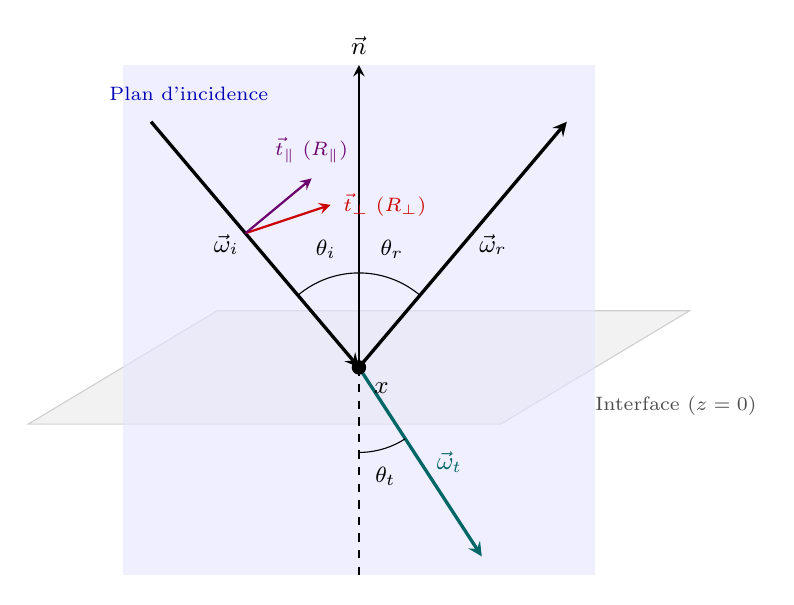
\begin{tikzpicture}[scale=1.2, >=stealth]
        % --- Interface matérielle (plan horizontal z = 0) ---
        \filldraw[fill=gray!15, draw=gray!50, opacity=0.7] 
            (-3.5, -0.6) -- (1.5, -0.6) -- (3.5, 0.6) -- (-1.5, 0.6) -- cycle;
        \node[gray!60!black, font=\scriptsize, right] at (2.4, -0.4) {Interface ($z=0$)};

        % Origine x
        \coordinate (O) at (0, 0);

        % --- Plan d'incidence (ombré en bleu translucide) ---
        \fill[blue!10, opacity=0.6] 
            (-2.5, 3.2) -- (2.5, 3.2) -- (2.5, -2.2) -- (-2.5, -2.2) -- cycle;
        \node[blue!70!black, font=\scriptsize] at (-1.8, 2.9) {Plan d'incidence};

        % --- Normale de surface ---
        \draw[thick, ->] (O) -- (0, 3.2) node[above, font=\small] {$\vec{n}$};
        \draw[thick, dashed] (0, 0) -- (0, -2.2);

        % --- Rayons lumineux ---
        % Rayon incident
        \draw[very thick, ->] (-2.2, 2.6) -- (O) node[midway, left=2pt, font=\small] {$\vec{\omega}_i$};
        % Rayon réfléchi
        \draw[very thick, ->] (O) -- (2.2, 2.6) node[midway, right=2pt, font=\small] {$\vec{\omega}_r$};
        % Rayon réfracté (transmis)
        \draw[very thick, ->, teal!80!black] (O) -- (1.3, -2.0) node[midway, right=2pt, font=\small] {$\vec{\omega}_t$};

        % --- Angles theta_i, theta_r, theta_t ---
        \draw[thin] (0, 1.0) arc (90:130:1.0);
        \node[font=\footnotesize] at (-0.35, 1.25) {$\theta_i$};

        \draw[thin] (0, 1.0) arc (90:50:1.0);
        \node[font=\footnotesize] at (0.35, 1.25) {$\theta_r$};

        \draw[thin] (0, -0.9) arc (-90:-57:0.9);
        \node[font=\footnotesize] at (0.28, -1.15) {$\theta_t$};

        % --- Décomposition de la polarisation sur le rayon incident ---
        \coordinate (P) at (-1.2, 1.42); % Point sur le rayon incident

        % Axe perpendiculaire (t_perp : hors du plan, le long de l'interface)
        \draw[thick, ->, red!80!black] (P) -- ++(0.9, 0.3) 
            node[right=1pt, font=\scriptsize] {$\vec{t}_\perp$ ($R_\perp$)};

        % Axe parallèle (t_parallel : dans le plan d'incidence, orthogonal au rayon)
        \draw[thick, ->, violet!85!black] (P) -- ++(0.7, 0.58) 
            node[above=2pt, font=\scriptsize] {$\vec{t}_\parallel$ ($R_\parallel$)};

        % Point de contact
        \filldraw[fill=black] (O) circle (2pt) node[below right=2pt, font=\small] {$x$};
    \end{tikzpicture}
    \caption{Décomposition des composantes de polarisation orthogonale ($R_\perp$) et parallèle ($R_\parallel$) par rapport au plan d'incidence.}
    \label{fig:fresnel_polarisation_schema}
\end{figure}

